%!TEX TS-program = xelatex

\documentclass[a4paper,12pt]{article}

%%% Работа с русским языком
\usepackage[english,russian]{babel}   %% загружает пакет многоязыковой вёрстки
\usepackage{fontspec}      %% подготавливает загрузку шрифтов Open Type, True Type и др.
\defaultfontfeatures{Ligatures={TeX},Renderer=Basic}  %% свойства шрифтов по умолчанию
\setmainfont[Ligatures={TeX,Historic}]{Calibri} %% задаёт основной шрифт документа
\setsansfont{Comic Sans MS}                    %% задаёт шрифт без засечек
\setmonofont{Courier New}
\usepackage{indentfirst}
\frenchspacing

\renewcommand{\epsilon}{\ensuremath{\varepsilon}}
\renewcommand{\phi}{\ensuremath{\varphi}}
\renewcommand{\kappa}{\ensuremath{\varkappa}}
\renewcommand{\le}{\ensuremath{\leqslant}}
\renewcommand{\leq}{\ensuremath{\leqslant}}
\renewcommand{\ge}{\ensuremath{\geqslant}}
\renewcommand{\geq}{\ensuremath{\geqslant}}
\renewcommand{\emptyset}{\varnothing}

%%% Дополнительная работа с математикой
\usepackage{amsmath,amsfonts,amssymb,amsthm,mathtools} % AMS
\usepackage{icomma} % "Умная" запятая: $0,2$ --- число, $0, 2$ --- перечисление

%% Номера формул
%\mathtoolsset{showonlyrefs=true} % Показывать номера только у тех формул, на которые есть \eqref{} в тексте.
%\usepackage{leqno} % Нумерация формул слева	

%% Перенос знаков в формулах (по Львовскому)
\newcommand*{\hm}[1]{#1\nobreak\discretionary{}
	{\hbox{$\mathsurround=0pt #1$}}{}}

%%% Работа с картинками
\usepackage{graphicx}  % Для вставки рисунков
\graphicspath{{images/}}  % папки с картинками
\setlength\fboxsep{3pt} % Отступ рамки \fbox{} от рисунка
\setlength\fboxrule{1pt} % Толщина линий рамки \fbox{}
\usepackage{wrapfig} % Обтекание рисунков текстом

%%% Работа с таблицами
\usepackage{array,tabularx,tabulary,booktabs} % Дополнительная работа с таблицами
\usepackage{longtable}  % Длинные таблицы
\usepackage{multirow} % Слияние строк в таблице
\usepackage{float}% http://ctan.org/pkg/float

%%% Программирование
\usepackage{etoolbox} % логические операторы


%%% Страница
\usepackage{extsizes} % Возможность сделать 14-й шрифт
\usepackage{geometry} % Простой способ задавать поля
\geometry{top=20mm}
\geometry{bottom=20mm}
\geometry{left=30mm}
\geometry{right=15mm}
%
%\usepackage{fancyhdr} % Колонтитулы
% 	\pagestyle{fancy}
%\renewcommand{\headrulewidth}{0pt}  % Толщина линейки, отчеркивающей верхний колонтитул
% 	\lfoot{Нижний левый}
% 	\rfoot{Нижний правый}
% 	\rhead{Верхний правый}
% 	\chead{Верхний в центре}
% 	\lhead{Верхний левый}
%	\cfoot{Нижний в центре} % По умолчанию здесь номер страницы

\usepackage{setspace} % Интерлиньяж
\onehalfspacing % Интерлиньяж 1.5
%\doublespacing % Интерлиньяж 2
%\singlespacing % Интерлиньяж 1

\usepackage{lastpage} % Узнать, сколько всего страниц в документе.

\usepackage{soul} % Модификаторы начертания

\usepackage{hyperref}
\usepackage[usenames,dvipsnames,svgnames,table,rgb]{xcolor}
\hypersetup{				% Гиперссылки
	unicode=true,           % русские буквы в раздела PDF
	pdftitle={Отчет о прохождении практики},   % Заголовок
	pdfauthor={Самоделкина М.В.},      % Автор
	pdfsubject={Отчет о прохождении практики},      % Тема
	pdfcreator={Самоделкина М.В.}, % Создатель
	pdfproducer={Самоделкина М.В.}, % Производитель
	pdfkeywords={keyword1} {key2} {key3}, % Ключевые слова
	colorlinks=true,       	% false: ссылки в рамках; true: цветные ссылки
	linkcolor=blue,          % внутренние ссылки
	citecolor=black,        % на библиографию
	filecolor=magenta,      % на файлы
	urlcolor=blue           % на URL
}
\makeatletter 
\def\@biblabel#1{#1. } 
\makeatother
\usepackage{cite} % Работа с библиографией
%\usepackage[superscript]{cite} % Ссылки в верхних индексах
%\usepackage[nocompress]{cite} % 
\usepackage{csquotes} % Еще инструменты для ссылок

\usepackage{multicol} % Несколько колонок

\usepackage{tikz} % Работа с графикой
\usepackage{pgfplots}
\usepackage{pgfplotstable}

% ГОСТ заголовки
\usepackage[font=small]{caption}
%\captionsetup[table]{justification=centering, labelsep = newline} % Таблицы по правобу краю
%\captionsetup[figure]{justification=centering} % Картинки по центру
\usepackage{ dsfont }

\newcommand{\tablecaption}[1]{\addtocounter{table}{1}\small \begin{flushright}\tablename \ \thetable\end{flushright}%	
\begin{center}#1\end{center}}

\newcommand{\imref}[1]{рис.~\ref{#1}}

\usepackage{multirow}
\usepackage{spreadtab}
\newcolumntype{K}[1]{@{}>{\centering\arraybackslash}p{#1cm}@{}}


\usepackage{xparse}
\usepackage{fancyvrb}

\RecustomVerbatimCommand{\VerbatimInput}{VerbatimInput}
{
	fontsize=\footnotesize    
}

\newcolumntype{?}[1]{!{\vrule width #1}}

\usepackage{tocloft}
\renewcommand{\cftsecleader}{\cftdotfill{\cftdotsep}}

\usepackage{pdfpages}

\usepackage{longtable}
\begin{document} % конец преамбулы, начало документа
\begin{titlepage}
	\begin{center}
		ПРАВИТЕЛЬСТВО РОССИЙСКОЙ ФЕДЕРАЦИИ \\
 		ФЕДЕРАЛЬНОЕ  ГОСУДАРСТВЕННОЕ АВТОНОМНОЕ \\
		ОБРАЗОВАТЕЛЬНОЕ УЧРЕЖДЕНИЕ ВЫСШЕГО ОБРАЗОВАНИЯ\\
		«НАЦИОНАЛЬНЫЙ ИССЛЕДОВАТЕЛЬСКИЙ УНИВЕРСИТЕТ\\
		«ВЫСШАЯ ШКОЛА ЭКОНОМИКИ»
	\end{center}
	
	\begin{center}
		\textbf{Московский институт электроники и математики}
		
		\textbf{Им. А.Н.Тихонова НИУ ВШЭ}
		
		\vspace{2ex}
		
		\textbf{Направление 01.03.04. Прикладная математика \\
			Бакалаврская программа <<Прикладная математика>>}
	\end{center}
	\vspace{1ex}	
	
	\vspace{1ex}
	\begin{center}
		\textbf{Отчет по самостоятельной работе \\
			по дисциплине <<Методы анализа стохастических взаимосвязей>>\\
			часть 1
	}
	\end{center}	

	\vspace{2ex}
	\vfill
	
	\vspace{2ex}
	
	\begin{flushright}
		\textbf{Бригада №7:}
		
		\vspace{2ex}
		
		Ремизова Анна Петровна, 4 курс, БПМ174
		
		Самоделкина Мария Владимировна, 4 курс, БПМ174

	\end{flushright}

	\vspace{5ex}
	\begin{center}
		Москва \the\year \, г.
	\end{center}
	
\end{titlepage}
\addtocounter{page}{1}
%\title{Отчет о прохождении производственной практики}
%\date{}
%\maketitle
%\includepdf{data/title2.pdf}
\tableofcontents
\pagebreak

\section{Общая постановка задачи}
\subsection{Формулировка прикладной проблемы}
В настоящее время в связи со сложной эпидемиологической обстановкой в мире очень актуально медицинское страхование. В частности США является лидером по заболеваемости от COVID-19 по информации с сайта Всемирной Организации Здравоохранения. Как известно, медицинское обслуживание в этой стране имеет страховой характер. По данным сайта переписи населения США 91,5\% населения США имеет медицинскую страховку. Следовательно, большая часть людей заинтересованы в ее приобретении. При этом размер страхового взноса зависит от параметров потребителя, и чаще всего вычисляется индивидуально. В связи с этим для актуария встает проблема определения размера страхового взноса для разных категорий населения.

В данной работе рассматривается задача определения размера минимального индивидуального взноса для конкретной категории населения, а именно
для некурящих женщин в возрасте 19–44 лет с индексом массы тела в диапазоне от 18,5 до 25 при наличии двух детей. Наш выбор обосновывается тем, что по статистике женщины на 32\% чаще мужчин берут страховку, а остальные параметры соответствуют среднестатистическому здоровому человеку.
%Определение размера индивидуальных взносов медицинского страхования по информации о человеке: полу, возрасту, индексу массы тела, количеству детей, наличию вредных привычек и региону.

\subsection{Потенциальные потребители решения. Задачи, которые они смогут решать,	используя полученные результаты}
Полученные решения будут применяться медицинскими страховыми компаниями в США. Набор данных соответствует северным районам США - в них находятся мегалополисы с большой численностью населения.

Используя полученные результаты, потребители смогут оценивать размер индивидуальных взносов, основываясь на индивидуальных характеристиках человека.

\subsection{Основные гипотезы, которые планируется проверить в рамках решения задачи}
В таблице \ref{tab:table1} представлены индивидуальные характеристики человека, используемые для анализа медицинских взносов. 

\begin{table}[H]
\begin{center}
	\begin{tabular}{ | l | p{4cm} | p{2.6cm} | p{4.2cm} | p{3.7cm} |}
		\hline
		№ & Характеристика объекта & Название переменной & Шкала измерения & Роль переменной \\ \hline
		1 & Возраст & age & Относительная & Независимая \\ \hline
		2 & Пол & sex & Номинальная (дихотомическая) & Независимая \\ \hline
		3 & Индекс массы тела & bmi & Относительная & Независимая \\ \hline
		4 & Число детей & children & Порядковая & Независимая \\ \hline
		5 & Наличие вредных привычек (курение) & smoker & Номинальная (дихотомическая) & Независимая \\ \hline
		6 & Индивидуальные годовые взносы (в долларах) & charges & Относительная & Зависимая \\ \hline
	\end{tabular}
\end{center}
\caption{Описание факторов, учтенных в анализе.}
\label{tab:table1}
\end{table}
Сформулируем гипотезы о статистической взаимосвязи зависимых и независимых переменных:
\begin{enumerate}
	\item У людей с вредными привычками размер страховых взносов больше, чем у людей без вредных привычек. Это обосновывается тем, что у курящих людей вероятность заболеваний дыхательных путей выше, что приводит к страховым случаям.
	%\item Индекс массы тела человека до некоторого возраста растет, а затем уменьшается.
	
	\item С ростом индекса массы тела, после некоторого значения, сила его влияния увеличивается. Это связывается с тем, что люди с чрезмерно высоким весом чаще подвержены заболеваниям сердечно-сосудистой системы. 
	%\item Цена медицинской страховки уменьшается с увеличением индекса массы тела до 18.5, затем размер взносов практически не меняется в зависимости от индекса массы тела в промежутке от 18,5 до 25, а затем с увеличением индекса снова растет. Это связывается с тем, что люди с чрезмерно низким и высоким весом чаще подвержены заболеваниям сердечно-сосудистой системы. 
	
	\item С возрастом размер медицинских страховых взносов растет. При этом скорость роста взносов у мужчин с возрастом выше, чем у женщин. Эта гипотеза подкреплена тем, что по статистике у пожилых людей больше хронических заболеваний и выше вероятность их обострения. При этом средняя продолжительность жизни женщин выше, чем у мужчин, что также отражается на частоте страховых случаев.
\end{enumerate}

\subsection{Основные источники данных}
Основные источники данных, использованные в работе.
\begin{enumerate}
	\item Данные были взяты из \href{https://github.com/stedy/Machine-Learning-with-R-datasets/blob/master/insurance.csv}{репозитория в GitHub};
	\item Информация по заболеваемости COVID-19 доступна на \href{https://covid19.who.int/}{сайте Всемирной Организации Здравоохранения};
	\item Интервал нормы индекса массы тела здорового человека нашли на  \href{https://www.cdc.gov/healthyweight/assessing/bmi/adult_bmi/index.html}{сайте департамента здоровья США};
	\item Статистика по процентам застрахованного населения США взята с \href{https://www.census.gov/library/publications/2019/demo/p60-267.html#:~:text=The%20percentage%20of%20people%20with,in%202017%20(92.1%20percent).}{официального сайта переписи населения США}.
	\item Различия по частоте страхования между мужчинами и женщинами и выделение возрастной группы женщин взяты из статьи Cylus J. et al. Pronounced gender and age differences are evident in personal health care spending per person //Health Affairs. – 2011. – Т. 30. – №. 1. – С. 153-160.
	
\end{enumerate}

\section{Предварительный анализ собранных данных}
\subsection{Анализ особенностей данных}
\subsubsection{Анализ количественных переменных}

\begin{table}[H]
	\begin{center}
		\begin{tabular}{|l|r@{,}l|r@{,}l|r@{,}l|r@{,}l|}
			\hline
			Переменная & \multicolumn{2}{c|}{Среднее}
			& \multicolumn{2}{c|}{Медиана}
			& \multicolumn{2}{c|}{Минимум}
			& \multicolumn{2}{c|}{Максимум} \\[1ex]
			\hline
			age & 39&233 & 39&000 & 18&000 & 64&000\\
			bmi & 29&187 & 28&880 & 15&960 & 48&070\\
			charges & 12911& & 9644&3 & 1621&3 & 60021&\\[10pt]
			\hline
			Переменная &  \multicolumn{2}{c|}{Ст.\ Откл.}
			& \multicolumn{2}{c|}{Вариация}
			& \multicolumn{2}{c|}{Асимметрия}
			& \multicolumn{2}{c|}{Эксцесс} \\[1ex]
			\hline
			age & 14&050 & 0&35811 & 0&051080 & $-$1&2547\\
			bmi & 5&5467 & 0&19004 & 0&15599 & $-$0&25062\\
			charges & 11167& & 0&86488 & 1&5758 & 2&1084\\[10pt]
			\hline
			Переменная &  \multicolumn{2}{c|}{5\% проц.}
			& \multicolumn{2}{c|}{95\% проц.}
			& \multicolumn{2}{c|}{IQ Range}
			& \multicolumn{2}{c|}{Пропущенные наблюдения} \\[1ex]
			\hline
			age & 18&500 & 61&500 & 25&000 & \multicolumn{2}{c|}{0}\\
			bmi & 19&998 & 39&045 & 7&5525 & \multicolumn{2}{c|}{0}\\
			charges & 2135&9 & 39661& & 11043& & \multicolumn{2}{c|}{0}\\
			\hline
		\end{tabular}
	\end{center}
	\caption{Описательные статистики количественных переменных.}
	\label{tab:table2}
\end{table}

\begin{figure}[H]
	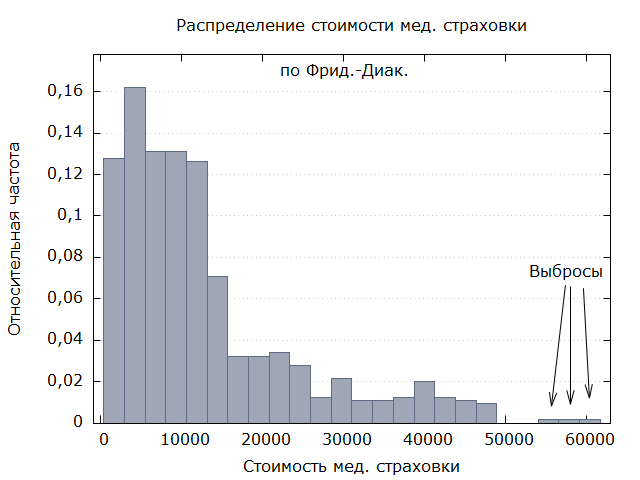
\includegraphics[width=0.6\textwidth]{../[graphics]/charges.png}
	\centering
	\caption{Стоимость страховки}
	\label{fig:charges}
\end{figure}

На основании анализа гистограммы рис. \ref{fig:charges} и описательных статистик табл. \ref{tab:table2} следует сделать вывод о том, что распределение целевой переменной асимметрично вправо. Это объясняется тем, что основная часть клиентов платит относительно средние суммы. Но есть и другая группа людей с повышенными медицинскими рисками, их не так много, но цена страховки для них выше. Хвост распределения очень длинный, это объясняется тем, что наблюдается большая вариативность в стоимости страховки. Есть выбросы с заметно большей стоимостью медицинской страховки, их доля очень мала. Полимодальности нет, естественной группировки нет.

\begin{figure}[H]
	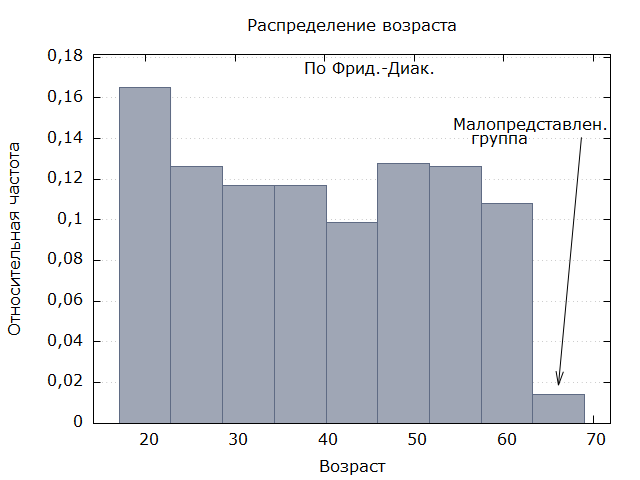
\includegraphics[width=0.6\textwidth]{../[graphics]/age.png}
	\centering
	\caption{Возраст}
	\label{fig:age}
\end{figure}

Распределение возраста (рис. \ref{fig:age}, табл. \ref{tab:table2}) асимметрично вправо. По виду гистограммы можно говорить о наличии двух кластеров: молодых людей в возрасте от 18 до 23 лет и людей, старше 23 лет. Респонденты в возрасте 18-23 лет резко выделяются, они широко представлены в выборке. Это отражает особенность системы страхования: у молодых людей заканчивается детская страховка и они массово оформляют взрослый вариант впервые. Остальные группы возрастов равно представленны. Это отражает свойство генеральной совокупности, а именно, что представители каждого возраста имеют одинаковый процент застрахованных, который практически неизменен, люди продлевают страховку из года в год. Группа людей в возрасте от 63 до 69 лет малопредставленна, что частично отражает свойство генеральной совокупности, так как часть людей не доживает до такого возраста. Также малопредставленность может быть обусловлена тем, что люди пожилого возраста не берут страховку, поскольку она для них дорогая и они не могут себе ее позволить. В свою очередь страховщики неохотно оформляют или оформляют по завышенной цене медицинскую страховку из-за больших рисков потерять средства. Следовательно, полимодальность есть.

\begin{figure}[H]
	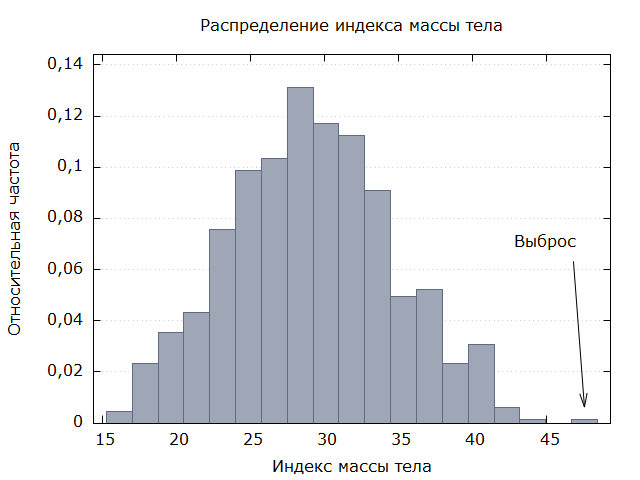
\includegraphics[width=0.6\textwidth]{../[graphics]/bmi.png}
	\centering
	\caption{Индекс массы тела}
	\label{fig:bmi}
\end{figure}

На основании анализа гистограммы рис. \ref{fig:charges} и описательных статистик табл. \ref{tab:table2} следует сделать вывод о том, что распределение индекса массы тела близко к нормальному, с незначительной правосторонней асимметрией. Действительно, согласно последним исследованиям, среди американцев преобладают люди с избыточной массой тела. Ниже в табл. \ref{tab:bmi} представлена интерпретация ИМТ в соответствии с рекомендациями ВОЗ.

\begin{table}[H]
	\begin{center}
		\begin{tabular}{ | l | l |}
			\hline
			ИМТ & Интерпретация \\ \hline
			Менее 18,5 & Дефицит массы тела \\ \hline
			18,5 - 24,9 & Норма \\ \hline
			25,0 - 29,9 & Избыточная масса тела \\ \hline
			Более 30,0 & Ожирение \\ \hline
		\end{tabular}
	\end{center}
	\caption{Интерпретация ИМТ в соответствии с рекомендациями ВОЗ.}
	\label{tab:bmi}
\end{table}

Медиана и среднее находятся в диапазоне избыточной массы тела, что также подтверждает свойства генеральной совокупности.

Кроме того, хорошо заметен выброс с аномально большой массой тела, что также согласуется с действительностью.

\subsubsection{Анализ качественных переменных}

\begin{figure}[H]
	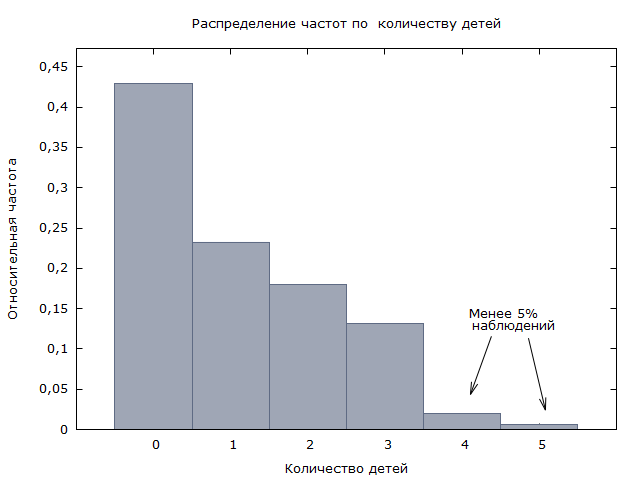
\includegraphics[width=0.6\textwidth]{../[graphics]/children.png}
	\centering
	\caption{Количество детей}
	\label{fig:children}
\end{figure}

По распределению частот количества детей (рис. \ref{fig:children}) можно отметить, что группы респондентов с 4 и 5 детьми достаточно малы (составляют менее 5\% наблюдений), поэтому предлагается агрегировать категории 3, 4 и 5 делей в одну категорию "3 и более детей". Результат приведён на распределении частот количества детей на рис. \ref{fig:children_agr}.

\begin{figure}[H]
	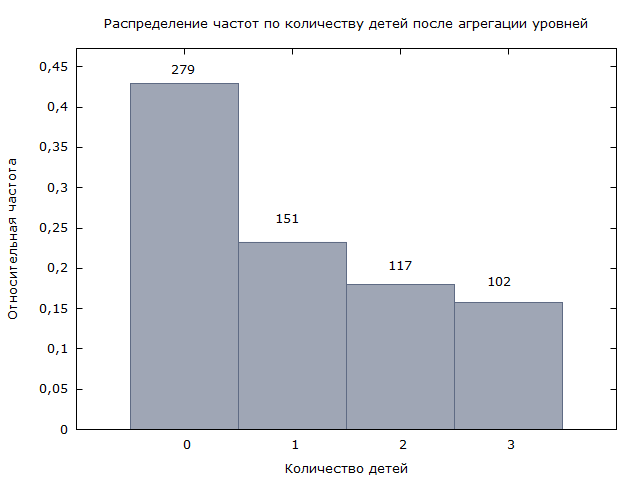
\includegraphics[width=0.6\textwidth]{../[graphics]/children_agr.png}
	\centering
	\caption{Количество детей после агрегации уровней}
	\label{fig:children_agr}
\end{figure}

Теперь все категории представлены более, чем 5\% данных, выборка является сбалансированной. Категория 3 обозначает "3 и более детей". Соотношение групп отражает реальную ситуацию в Америке: больше всего людей без детей, а с увеличением количества детей уменьшается количество людей из таких семей.

\begin{figure}[H]
	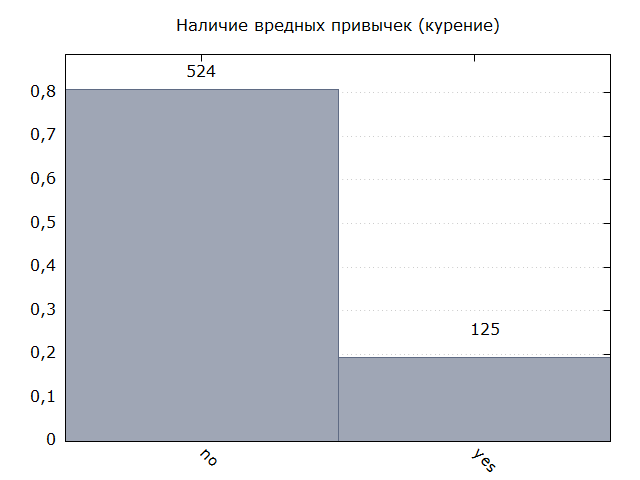
\includegraphics[width=0.6\textwidth]{../[graphics]/smoker.png}
	\centering
	\caption{Наличие вредных привычек}
	\label{fig:smoker}
\end{figure}

По признаку наличия вредных привычек выборка не является сбалансированной (рис. \ref{fig:smoker}), что есть естественное свойство генеральной совокупности: в действительности некурящих людей больше, чем курящих. Агрегацию уровней проводить не требуется, группы курящих и некурящих людей не являются малопредставленными.

\begin{figure}[H]
	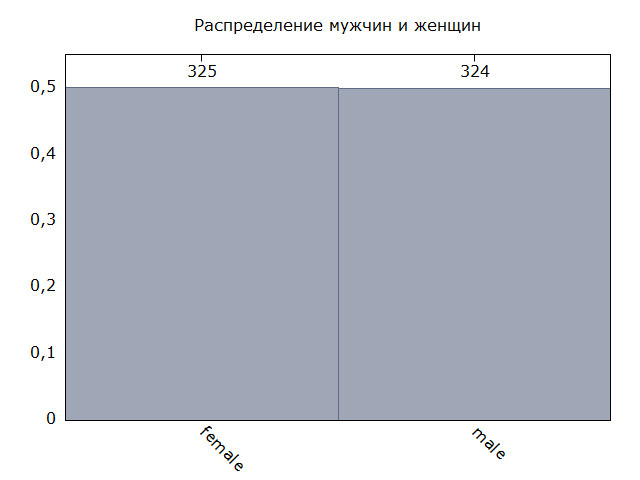
\includegraphics[width=0.6\textwidth]{../[graphics]/sex.png}
	\centering
	\caption{Пол}
	\label{fig:sex}
\end{figure}

Выборка сбалансирована по полу - представлено равное количество мужчин и женщин. Это отражает репрезентативность выборки.

\subsubsection{Анализ репрезентативности выборки}

В качестве итога анализа качественных и количественных переменных можно сказать, что выборка не смещена и отражает естественные свойства генеральной совокупности.

\subsection{Анализ статистической связи}

\subsubsection{Графический анализ пары «числовая зависимая переменная – качественная независимая переменная»}

\begin{figure}[H]
	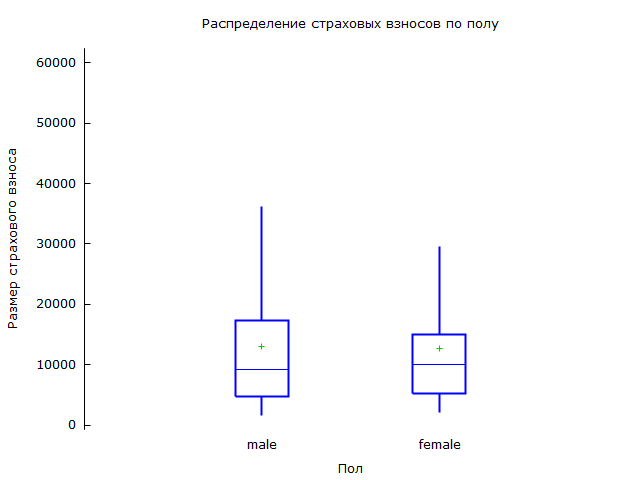
\includegraphics[width=0.6\textwidth]{../[graphics]/charges-sex.png}
	\centering
	\caption{Зависимость страховых взносов от пола}
	\label{fig:charges-sex}
\end{figure}

По представленной на рис. \ref{fig:charges-sex} диаграмме <<ящик с усами>> видно, что, в среднем, размер страховых выплат не зависит от пола. Однако, есть некоторые различия между подвыборками мужской и женской половины населения. Во-первых, максимальные размер страховых выплат - у мужчин, и он значительно больше, чем у женщин. Во-вторых, медиана страховых выплат среди мужчин смещена к первому квартилю, в то время, как у женщин медиана находится ровно посередине. В-третьих, среди мужчин разброс величины страховых больше, чем среди женщин.

Для рассматриваемой пары переменных был проведён тест Краскела — Уоллиса с целью формальной проверки гипотезы о статистической взаимосвязи. Было получено значение p-value $0,45 > 0,05$ - значит гипотезу $H_0$ об отсутствии значимых отличий между выплатами для мужчин и для женщин не отвергаем на уровне значимости $5\%$.

\begin{figure}[H]
	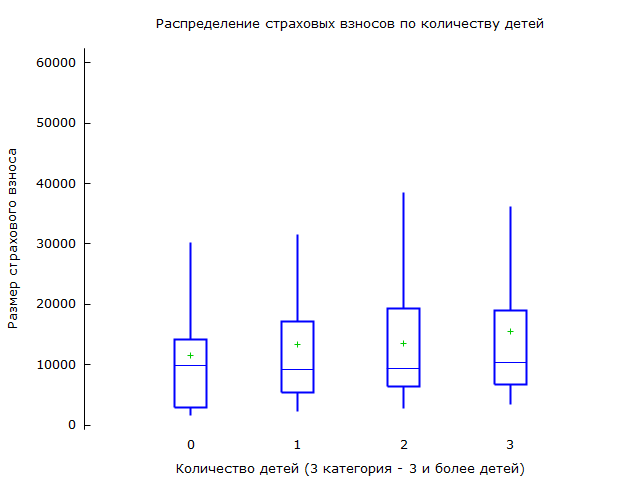
\includegraphics[width=0.6\textwidth]{../[graphics]/charges-children_agr.png}
	\centering
	\caption{Зависимость страховых взносов от количества детей}
	\label{fig:charges-children_agr}
\end{figure}

По представленной на рис. \ref{fig:charges-children_agr} диаграмме <<ящик с усами>> видно, что, в среднем, размер страховых взносов имеет тенденцию к увеличеснию с увеличением количества детей в семье. При этом медиана при переходе от уровня к уровню изменяется незначительно. При изменении количества детей от 0 до 3 наблюдается смещение диапазона страховых выплат в сторону более высоких значений, а для респондентом в большим количеством детей (3 и более) диапазон возвращается к значениям выплат группы респондентов с 2 детьми.

\begin{figure}[H]
	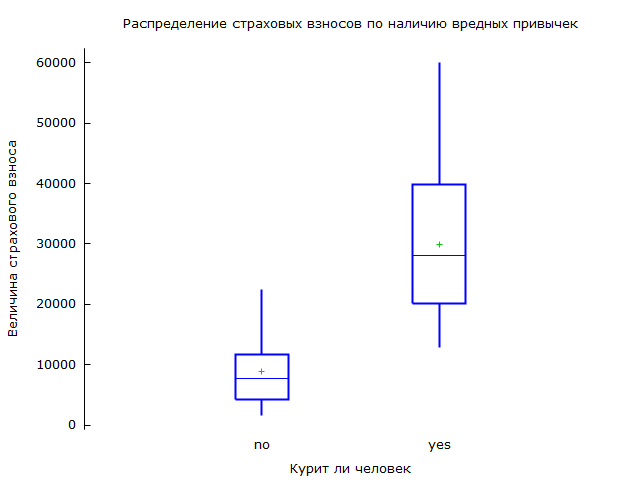
\includegraphics[width=0.6\textwidth]{../[graphics]/charges-smoker.png}
	\centering
	\caption{Зависимость страховых взносов от курения}
	\label{fig:charges-smoker}
\end{figure}

На диаграмме <<ящик с усами>> (рис. \ref{fig:charges-smoker}) хорошо заметно, что, в среднем, для курящих людей размер страховых выплат больше, чем для некурящих: и среднее, и медиана, и диапазон сдвинуты в сторону высоких значений выплат.

Для рассматриваемой пары переменных также был проведён тест Краскела — Уоллиса с целью формальной проверки гипотезы о статистической взаимосвязи. Было получено значение p-value $0,00 < 0,05$ - значит принимаем альтернативную гипотезу $H_1$ о наличии значимых отличий между выплатами для курящих и некурящих людей на уровне значимости $5\%$.

\subsubsection{Графический анализ пары «числовая зависимая переменная – числовая независимая переменная»}

\begin{figure}[H]
	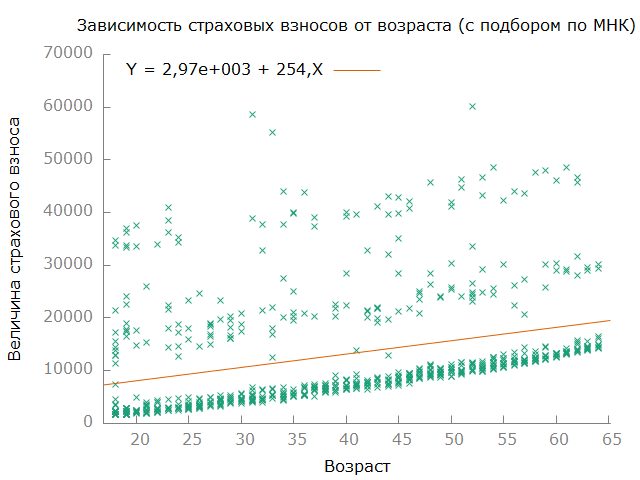
\includegraphics[width=0.6\textwidth]{../[graphics]/age-price.png}
	\centering
	\caption{Зависимость страховых взносов от возраста}
	\label{fig:age-price}
\end{figure}

Анализируя график на рисунке \ref{fig:age-price}, можно выделить 3 группы людей: здоровые люди (возможно некурящие, с небольшим индексом массы тела), группа с отклонениями в здоровье и группа людей со значительными отклонениями в здоровье (вероятно курящие и с ожирением). 

Для каждой такой группы людей видна явная линейная зависимость цены страховки от возраста. Причем коэффициент роста цены на страховку с возрастом визуально одинаковый для всех установленных групп людей. Множитель при возрасте в рассматриваемой линейной зависимости можно интерпретировать как надбавку в стоимости страховки за возраст. При этом цены на страховку в каждой группе людей сильно отличаются значением свободного коэффициента. Для здоровых людей этот коэффициент низкий, поскольку риски заболевания у них небольшие. Для остальных групп этот коэффициент будет выше, поскольку вероятность страхового случая для людей с отклонениями в здоровье значительно выше. 

Также стоит отметить, что разброс значений в стоимости страховки у первой группы людей значительно меньше, чем у других групп. Это объясняется тем, что в первой группе находятся здоровые люди: двум здоровым людям одного возраста положена страховка одинаковой стоимости, поскольку они по состоянию здоровья практически не отличаются. В это же время люди с отклонениями в здоровье могут иметь разные осложнения и разные степени заболевания, что сказывается и на стоимости.

На графике можно наблюдать выбросы, которые не описываются ни одной из обозначенных линейных зависимостей. При этом нет выбросов ниже линейной зависимости для первой группы людей. Действительно, абсолютно здоровому человеку страховщик не будет уменьшать цену, цена может только увеличиваться, если у человека есть какие-либо заболевания. 

\begin{figure}[H]
	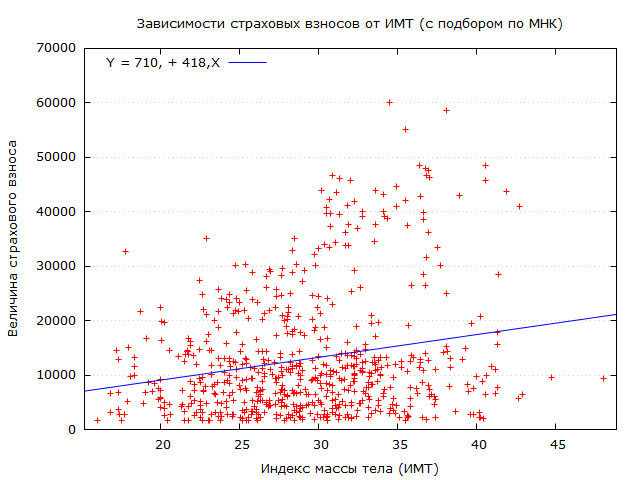
\includegraphics[width=0.6\textwidth]{../[graphics]/сharges-bmi.png}
	\centering
	\caption{Зависимость страховых взносов от индекса массы тела}
	\label{fig:charges-bmi}
\end{figure}

\begin{figure}[H]
	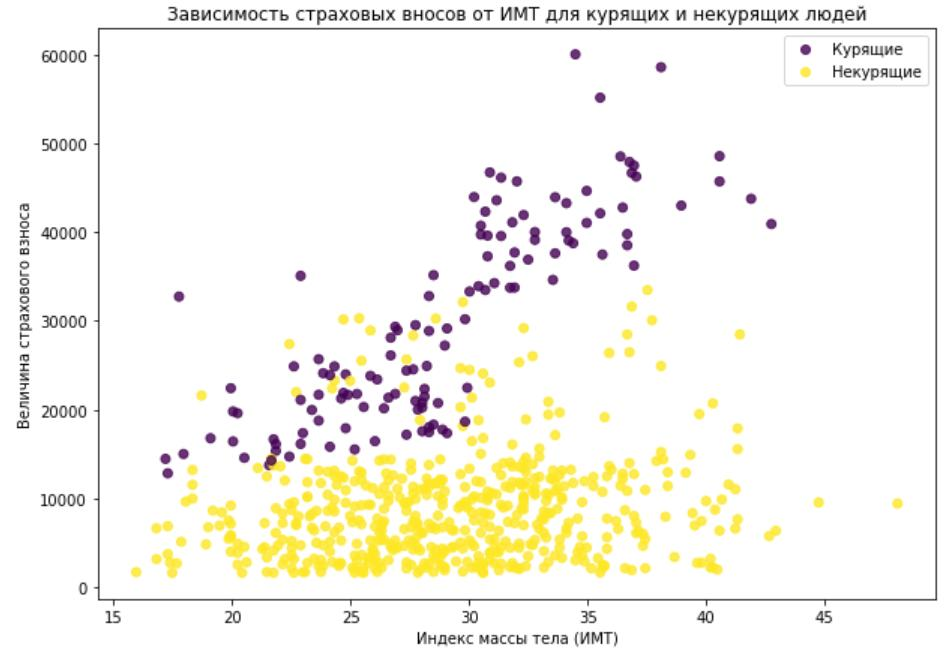
\includegraphics[width=0.6\textwidth]{../[graphics]/charges-bmi-smoker.jpg}
	\centering
	\caption{Зависимость страховых взносов от индекса массы тела для курящих и некурящих людей}
	\label{fig:charges-bmi-smoker}
\end{figure}

По диаграмме рассеяния на рисунке \ref{fig:charges-bmi} можно сделать вывод о том, что, в среднем, с увеличением индекса массы тела стоимость страховки увеличивается. На графике ясно видно наличие двух групп с разной скоростью роста страхового взноса в зависимости от ИМТ. В соответствии с рисунком \ref{fig:charges-bmi-smoker} можно предположить, что это группы курящих и некурящих людей. Однако зависимость не объясняется только линейной взаимосвязью: с увеличением ИМТ дисперсия страховых взносов возрастает. Это может быть связано с тем, что на здоровье людей без ожирения (с ИМТ $<30$, см. таблицу \ref{tab:bmi}) значение ИМТ практически не оказывает влияния, при этом люди с ожирением как могут не испытывать никаких осложнений, так и их здоровье может быть сильно хуже людей без ожирения - например, среди людей с ожирением более частыми являются случаи тяжёлых форм сердечно-сосудистых заболеваний.

\subsubsection{Анализ наличия корреляции между независимыми переменными}

\begin{table}[H]
	\begin{center}
		Таблица сопряженности Пол (строки) и Курение (столбцы)\\
		
		\vspace{8pt}
		
		\begin{tabular}{|l|l|l|l|}
			\hline
		    & Нет & Да & Всего \\[1ex]
		    \hline
			Женщина & $267$ & $58$ & $325$\\
			\hline
			Мужчина & $257$ & $67$ & $324$\\[1ex]
			\hline
			Всего & $524$ & $125$ & $649$\\
			\hline
		\end{tabular}
		\caption{Таблица кросс-табуляции между полом и курением}
		\label{tab:cross}
	\end{center}
\end{table}

По анализу таблицы сопряженности \ref{tab:cross} и значению статистики Хи-квадрат = $0,84$ с p-значением равным $0,36 > 0,05$ можно сказать, что статистически значимой связи между полом и курением нет (гипотезу $H_0$ об отсутствии значимой связи не отвергаем на уровне значимости $5\%$). Это ожидаемый результат, поскольку и мужчины, и женщины практически в равной степени подвержены формированию вредных привычек, в частности курению.

\begin{table}[H]
	\begin{center}
		Таблица сопряженности Пол (строки) и Число детей (столбцы)\\
		
		\vspace{8pt}
		
		\begin{tabular}{|l|l|l|l|l|l|}
			\hline
			& 0 & 1 & 2 & 3 и более & Всего \\[1ex]
			\hline
			Женщина & $135$ & $79$ & $56$ & $54$ & $324$\\
			\hline
			Мужчина & $144$ & $72$ & $61$ & $48$ & $325$\\[1ex]
			\hline
			Всего & $279$ & $151$ & $117$ & $102$ & $649$\\
			\hline
		\end{tabular}
		\caption{Таблица кросс-табуляции между полом и количеством детей}
		\label{tab:cross2}
	\end{center}
\end{table}

По таблице сопряженности \ref{tab:cross2} и значению статистики Хи-квадрат = $1,1799$ (3 ст. свободы, p-значение = $0,757828$) можем сделать вывод об отсутсвии связи между полом и количеством детей, а именно: гипотезу $H_0$ об отсутсвии значимой связи не отвергаем на уровне значимости $5\%$. Действительно, так как в большинстве семей есть и женщина, и мужчина, то для каждой конкретной семьи количесто детей равное вне зависимости от пола, а значит и для генеральной совокупости не должно наблюдаться значимой связи между  

\begin{table}[H]
	\begin{center}
		Таблица сопряженности Курение (строки) и Число детей (столбцы)\\
		
		\vspace{8pt}
		
		\begin{tabular}{|l|l|l|l|l|l|}
			\hline
			& 0 & 1 & 2 & 3 и более & Всего \\[1ex]
			\hline
			Нет & $229$ & $120$ & $97$ & $78$ & $524$\\
			\hline
			Да & $50$ & $31$ & $20$ & $24$ & $125$\\[1ex]
			\hline
			Всего & $279$ & $151$ & $117$ & $102$ & $649$\\
			\hline
		\end{tabular}
		\caption{Таблица кросс-табуляции между курением и количеством детей}
		\label{tab:cross3}
	\end{center}
\end{table}

Хи-квадрат = 2,02674 (3 ст. свободы, p-значение = 0,566876)

По таблице сопряженности \ref{tab:cross3} и значению статистики Хи-квадрат = $2,02674$ (3 ст. свободы, p-значение = $0,566876$) можем сделать вывод об отсутсвии связи между курением и количеством детей, а именно: гипотезу $H_0$ об отсутсвии значимой связи не отвергаем на уровне значимости $5\%$. Действительно, как курение не должно влиять на количество детей в генеральной совокупности, так и количество детей не должно влиять на наличие вредных привычек у человека.

Приведем таблицу с коэффициентами корреляции Пирсона для анализа силы связи между независимыми числовыми переменными. 

\begin{table}[H]
\begin{center}
	\vspace{8pt}
	\begin{tabular}{|r|r|l|}
		\hline
		Возраст & ИМТ &\\
		\hline
		$1,0000$ & $0,1324$ & Возраст\\
		\hline
		& $1,0000$ & ИМТ\\
		\hline
	\end{tabular}
	\caption{Таблица коэффициентов корреляции Пирсона}
	\label{tab:pris}
\end{center}
\end{table}

При анализе таблицы \ref{tab:pris} выявлена очень слабая корреляция. Значение t-статистики для $647$ наблюдений равно $3,39745$ p-value $0,0007 > 0,05$, гипотезу $H_0$ об отсутствии корреляции отвергаем на уровне значимости $5\%$.

%Несмотря на то, что с возрастом количество детей у одного и того же человека может только увеличиваться, явной статистической связи между этими переменными нет. Это можно объяснить тем, что срез мы берем не по конкретному человеку, а по группе населения, и возраст отдельного человека этой группы уже никак не будет статистически связан с его количеством детей. 

%Также для мужчин абсолютно естественно, что количество детей никак не связано с ИМТ. Но может быть так, что женщина после родов набирает вес. Поскольку такое наблюдается не у всех женщин и не обязательно после первых по счету родов, то зависимость между количеством детей и ИМТ также не является значимой.

\begin{figure}[H]
	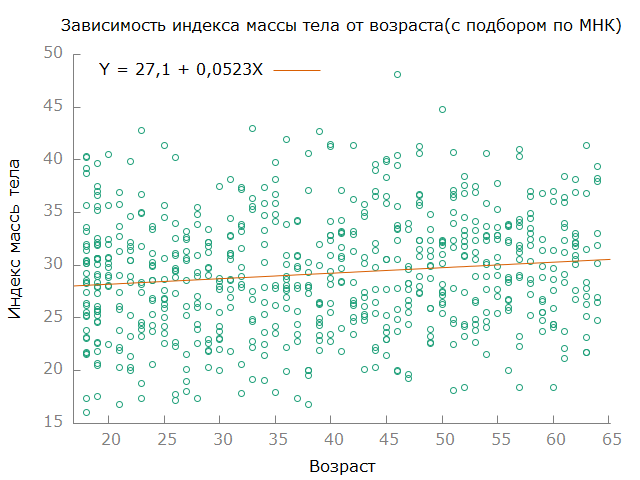
\includegraphics[width=0.6\textwidth]{../[graphics]/bmi-age.png}
	\centering
	\caption{Зависимость индекса массы тела от возраста}
	\label{fig:bmi-age}
\end{figure}

Действительно, у людей с увеличением возраста увеличивается и склонность к ожирению. Но при анализе диаграммы рассеяния (рис. \ref{fig:bmi-age}) видно, что явной и однозначной зависимости ИМТ от возраста нет, поскольку для каждого возраста виден достаточно широкий разброс в значениях ИМТ.
	
Значение критерия Краскела-Уоллиса для переменных возраста и пола chi-squared = $0,49$, p-value = $0,48 > 0,05$. Следовательно, нулевую гипотезу об отсутствии различий распределения возраста для мужчин и женщин не отвергаем на уровне значимости $5\%$. Полученный результат отражает свойство генеральной совокупности: с увеличением возраста пропорция мужчин и женщин в нормальных условиях (например, не военных) сохраняется. 

При проведении теста Краскела-Уоллиса для пола и ИМТ (chi-squared = $0,15$ и p-value = $0,70 > 0,05$) можно говорить об отсутствии статистической связи между полом человека и его ИМТ (гипотезу $H_0$ об отсутствии значимых различий не отвергаем на уровне значимости $5\%$). Данный результат ожидаем. Несмотря на то, что вес женщины обычно меньше веса мужчины, рост женщин в среднем также меньше, что компенсируется при вычислении ИМТ (рассчитывается как вес, деленный на квадрат роста).

%По значению критерия Краскела-Уоллиса для переменных количества детей и пола (chi-squared = $0,41$,  p-value = $0,52 > 0,05$) можно утверждать, что количество детей и пол человека статистически не связаны (гипотезу $H_0$ об отсутствии значимых различий не отвергаем на уровне значимости $5\%$). Это действительно так, ведь в среднестатистической семье (с обоими родителями разного пола) ребенок относится и к матери, и к отцу. Поскольку мужчин и женщин в нашем наборе данных примерно одинаковое количество, то количество детей человека не должно зависеть от пола.

Тест Краскела-Уоллиса для ИМТ и признака наличия вредных привычек со значениями chi-squared = $0,56$ и p-value = $0,45 > 0,05$ показывает, что зависимость между значеним ИМТ и привычной курения не связаны статистически (гипотезу $H_0$ об отсутствии значимых различий не отвергаем на уровне значимости $5\%$). Действительно, курение может влиять на здоровье как в сторону уменьшения, так и в сторону набора веса. Поэтому переменные статистически не связаны.

Значение критерия Краскела-Уоллиса для переменной возраста и признака наличия вредных привычек (chi-squared = $0,22$, p-value = $0,64 > 0,05$) показывает, что нулевая гипотеза об отсутствии различий распределения возраста для курящих и не курящих людей не отвергается на уровне значимости $5\%$. Это отражает свойство генеральной совокупности, ведь люди любого возраста одинаково подвержены приобретению вредных привычек.

%При проведении теста Краскела-Уоллиса для количества детей и наличия вредных привычек получаем значения chi-squared = $0,59$ и p-value = $0,44 > 0,05$ (гипотезу $H_0$ об отсутствии значимых различий не отвергаем на уровне значимости $5\%$). Это говорит о том, что различия распределения количества детей для курящих и не курящих людей нет.

Тест Краскела-Уоллиса для ИМТ и количества детей со значениями chi-squared = $2,9707$ и p-value = $0,70 > 0,05$ показывает, что зависимость между значеним ИМТ и количеством детей не связаны статистически (гипотезу $H_0$ об отсутствии значимых различий не отвергаем на уровне значимости $5\%$). Действительно, в большинстве случаев, ни ИМТ не влияет на возможность иметь большее или меньшее количество детей, ни количество детей, в среднем, не сказывается на ИМТ родителей.

Значение критерия Краскела-Уоллиса для переменной возраста и количества детей (chi-squared = $1,74$, p-value = $0,63 > 0,05$) показывает, что нулевая гипотеза об отсутствии различий распределения возраста для людей с разным количеством детей не отвергается на уровне значимости $5\%$. Это отражает свойство генеральной совокупности, и это связано с тем, что с возрастом, в целом, для конкретного человека количество детей может только не уменьшаться, но при этом в современном обществе всё большее и большее количество людей не имеет детей и не планирует их или останавливается на 1 ребёнке.

Итак, корреляции между независимыми переменными не выявлено, кроме очень слабой корреляции между ИМТ и возрастом.

\subsubsection{Предварительная проверка гипотез}

Гипотеза 1 о том, что у людей с вредными привычками размер страховых взносов больше, чем у людей без вредных привычек, подтверждается по результатам п. 2.2.1 - уже на диаграмме <<ящик с усами>> (рис. \ref{fig:charges-smoker}) отчётливо видно различие между рассматриваемыми группами людей. Численно результат подкреплён тестом Краскела-Уоллиса: альтернативная гипотеза о наличии значимых различий между размерами взносов курящих и некурящих людей была отвергнута на уровне значимости $5\%$.

Гипотеза 2 о различии влияния ИМТ на величину страхового взноса с ростом ИМТ подтверждается на основании рисунка \ref{fig:charges-bmi}: на диаграмме рассеяния видно, что приблизительно после значения ИМТ $= 30$ (порог ожирения) величина страховых выплат, в среднем, начинает расти сильнее при изменении ИМТ на 1, чем до значения ИМТ $= 30$. Это может быть связано с тем, что пока вес человека находится в пределах нормы, он не так сильно влияет на здоровье человека при изменениях, как вес людей с ожирением: чем больше вес (значение ИМТ), тем больше у человека может быть сопутствующих заболеваний, а также может увеличиваться тяжесть форм заболеваний.

Дополнительно была добавлена фиктивная переменная, равная $0$ при ИМТ $<30$ и $1$ при ИМТ $\ge30$. По диаграмме <<ящик с усами>> на рисунке \ref{fig:is_fat} уже более отчётливо видны структурные различия между двумя группами людей: с ожирением и без. Для людей с ожирением, в среднем, величина страховых выплат больше, а также диапазон выплат сдвинут в сторону более высоких значений. Формально, по тесту Краскела-Уоллиса, значение p-value $0,0018 < 0,05$, то есть принимается альтернативная гипотеза $H_1$ о наличии значимых различий между выплатами для людей с ожирением и без на уровне значимости $5\%.$

\begin{figure}[H]
	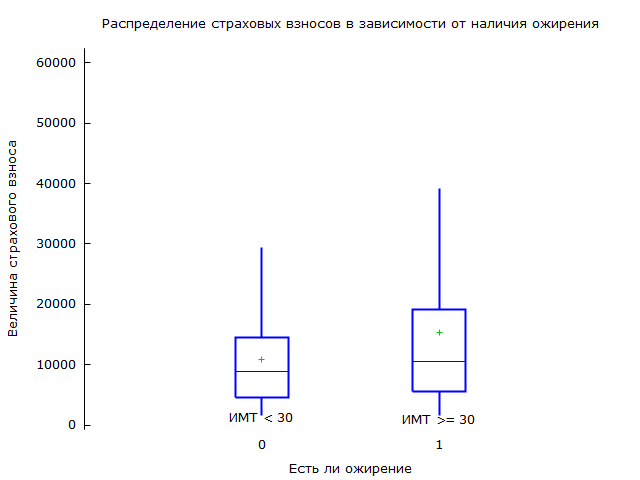
\includegraphics[width=0.6\textwidth]{../[graphics]/is_fat.png}
	\centering
	\caption{Зависимость величины страхового взноса от наличия ожирения}
	\label{fig:is_fat}
\end{figure}

Гипотеза 3 о том, что размер страховых выплат растёт с возрастом, также подтверждается на основании п. 2.2.2 (рис. \ref{fig:age-price}): на диаграмме рассеяния заметно практически линейное увеличение страховых взносов с возрастом для всей выборки. Для сравнения скорости роста величины страховых взносов у мужчин и у женщин необходим дополнительный анализ с пострением регрессионных моделей, что будет рассмотрено ниже.

\subsubsection{Дополнительные исследования}

При проведении нами дополнительных визуальных исследований хочется отметить несколько закономерностей, которые были выявлены.

\begin{figure}[H]
	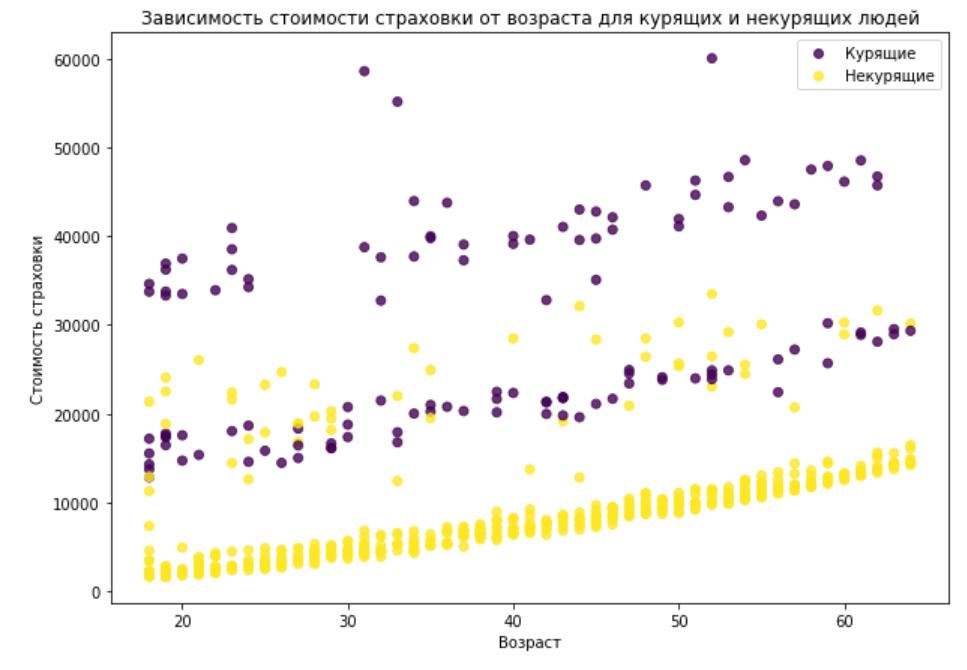
\includegraphics[width=0.7\textwidth]{../[graphics]/age-charges-smoker.jpg}
	\centering
	\caption{Зависимость цены страховки от возраста для курящих и некурящих людей}
	\label{fig:age-charges-smoker}
\end{figure}

Как видно из рисунка \ref{fig:age-charges-smoker} к первой группе (ранее охарактеризованной нами как здоровых людей) относятся только некурящие люди, а в третьей группе людей со значительными отклонениями в здоровье находятся только курящие люди.

\begin{figure}[H]
	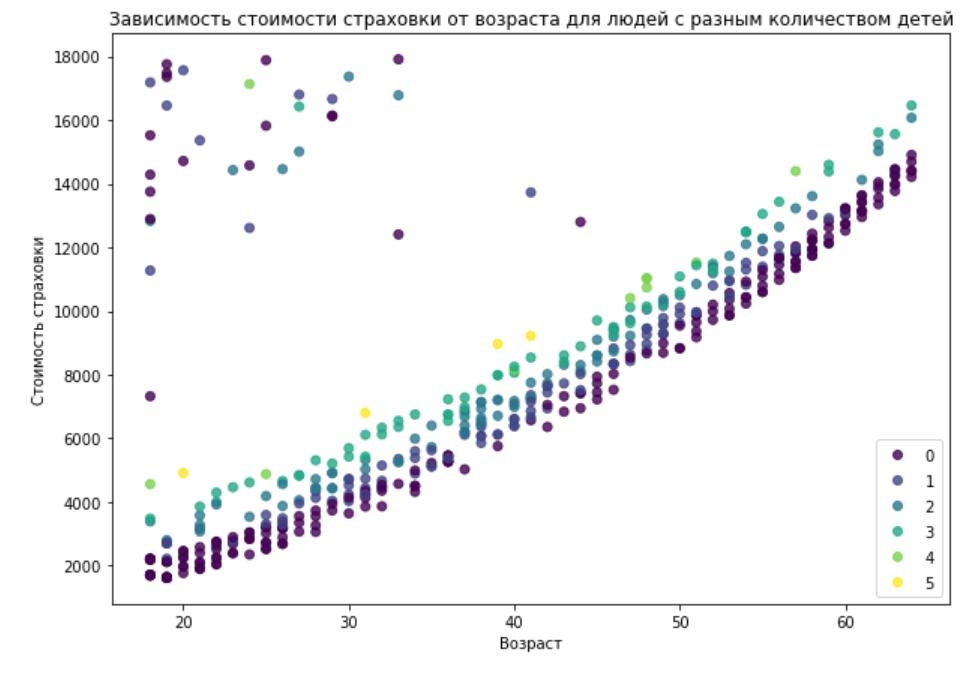
\includegraphics[width=0.7\textwidth]{../[graphics]/age-charges-childern.jpg}
	\centering
	\caption{Зависимость цены страховки от возраста для людей с разным количеством детей}
	\label{fig:age-charges-children}
\end{figure}

Рассмотрим детально график зависимости цены страховки от возраста для людей с разным количеством детей (рис. \ref{fig:age-charges-children}) для первой (здоровой) группы людей (на графике для наглядности изображены только точки со значением стоимости страховки меньше 18 тысяч). Видно, что чем больше у человека детей, тем дороже у него страховка в рамках первой группы людей. Для других групп данная закономерность не выполняется.

\section{Спецификация, оценивание и оптимизация модели}

\subsection{Спецификация моделей для проверки гипотез и решения поставленной задачи}

В качестве базовой модели используется регрессионная модель с линейным включением всех переменных кроме переменной $sex$, поскольку она не имеет значимой корреляционной связи с зависимой переменной и, хотя бы, с одной независимой. 

Выборка разделяется случайным образом на обучающую ($80\%$ от общего объема) для построения модели и тестовую ($20\%$) для проверки прогностических свойств. Также сделаем из переменной $smoker$ dummy-переменную $Dsmoker\_2$: она равна 1, если человек курит, и 0 в противном случае.

Из категориальной переменной $children$ сделаем несколько dummy-переменных. Изначально включим в модель все полученные фиктивные переменные, кроме $Dchildren\_0$ (равна 1, если у человека нет детей), чтобы предотвратить избыточность. Переменная $Dchildren\_1$ (равна 1, если у человека только 1 ребенок) оказалась незначимой, поэтому в базовую модель ее также не включаем. 

Исходя из вышесказанного, уравнение регрессии записывается следующим образом:
\[charges = a_0 + a_1 * age + a_2 * bmi + a_3 * Dchildren\_2 + a_4 * Dchildren\_many + a_5 * Dsmoker\_2,\]	
где $charges$ - стоимость медицинской страховки,
$age$ - возраст,
$bmi$ - ИМТ,
$Dchildren\_2$ - фиктивная переменная, равная 1, если количество детей равно 2, и 0 иначе,
$Dchildren\_many$ - фиктивная переменная, равная 1, если количество детей больше или равно 3, и 0 иначе,
$Dsmoker\_2$ - индикатор наличия вредных привычек, коэффициенты $a_i$, $i=0..5$ - сила влияния (постоянная) соответствующего фактора на зависимую переменную $charges$.

Гипотезу 1 о том, что наличие вредных привычек статистически связано с увеличением цены на страховку, проверим следующим образом. Если гипотеза $H_0$ о том, что наличие вредных привычек не влияет на цену, верна, то коэффициент при переменной $Dsmoker\_2$ $a_5 = 0$. Если верна альтернативная гипотеза $H_1$ о том, что наличие вредных привычек влияет на цену в сторону ее увеличения, то $a_5 > 0$.

Гипотезу 3 о том, что увеличение возраста статистически связано с увеличением цены на страховку, проверим следующим образом. Если гипотеза $H_0$ о том, что возраст не влияет на цену, верна, то коэффициент при переменной $age$ $a_1 = 0$. Если верна альтернативная гипотеза $H_1$ о том, что рост возраста влияет на цену в сторону ее увеличения, то $a_1 > 0$.

Произведем модификацию базовой модели для проверки гипотезы 2 о том, что с увеличением ИМТ цена растет медленно, а после какого-то значения ИМТ цена начинает расти быстрее. Зададим переменную-индикатор $bmi\_ind = 1 (bmi >= 30) + 0 (bmi < 30)$. Пороговое значение ИМТ, равное 30, соответствует нижней границе ожирения. Тогда значение коэффициента при переменной $bmi$ зависит от переменной-индикатора $bmi\_ind$, то есть $a_2(bmi\_ind) = c_1 * bmi\_ind + c_2$. Выражение для регрессии перепишется в следующем виде:
\begin{align*}
	charges = a_0 + a_1 * age + c_1 * bmi\_ind * bmi + c_2 * bmi + a_3 * Dchildren\_2 + \\ + a_4 * Dchildren\_many + a_5 * Dsmoker\_2.
\end{align*}

Гипотезу 2 проверим по следующей методике. Если ИМТ влияет на цену в сторону ее увеличения, то $a_2(bmi\_ind) > 0$. Тогда если $bmi\_ind = 0$, то $c_2 > 0$. Иначе если $bmi\_ind = 1$, то $c_1 + c_2 > 0$. Следовательно, $c_1$ должен быть также больше 0 (сила влияния после переломного момента увеличивается). Так, если $c_1, c_2 > 0$, то гипотеза 2 подтверждается.

Для построения модифицированной модели введем новую переменную $bmi\_bmi\_ind = bmi\_ind * bmi$.

Вторую часть гипотезы 3 о том, что скорость роста величины страховых выплат среди мужчин выше, чем среди женщин, проверим отдельно. Для этого учтем, что коэффициент перед возрастом зависит от пола следующим образом: $a_1(sex) = b_1 * sex + b_2$, где $sex = 1$, если это мужчина, и $sex = 0$, если женщина. Запишем, что $a_1(sex) > 0$, поскольку возраст влияет на стоимость в сторону ее увеличения. Тогда если $sex = 0$, то $b_2 > 0$. Иначе при $sex = 1$ $b_1 + b_2 > 0$. Поскольку в гипотезе полагается, что сила влияния возраста на цену страховки у мужчин больше, чем у женщин, то $b_1 > 0$. Запишем выражение для регрессии, модифицировав модель гипотезы 2:
\begin{align*}
charges = a_0 +  b_1 * sex * age + b_2 * age + c_1 * bmi\_ind * bmi + c_2 * bmi + \\ + a_3 * Dchildren\_2 + a_4 * Dchildren\_many + a_5 * Dsmoker\_2.
\end{align*}

Для построения модифицированной модели введем новую переменную $sex\_age = sex * age$.

\subsection{Оценивание базовой модели и результаты проверки гипотез}
\begin{table}[H]
	\begin{center}	
		Base\_model:
		МНК, использованы наблюдения 1--518\\
		Зависимая переменная: charges\\
		\vspace{1em}
		\begin{tabular}{|l|r@{,}l|r@{,}l|r@{,}l|r@{,}l|r@{,}l|}
			\hline
			&
			\multicolumn{2}{c|}{Коэффициент} &
			\multicolumn{2}{c|}{Ст.\ ошибка} &
			\multicolumn{2}{c|}{$t$-статистика} &
			\multicolumn{2}{c|}{P-значение} &
			\multicolumn{2}{c|}{VIF} \\[1ex]
			\hline
			const &	$-$13130&9 & 1551&90 & $-$8&461 & 0&0000 & -& \\
			\hline
			age & 252&787 &	18&7150 & 13&51 & 0&0000 & 1&013 \\
			\hline
			bmi & 386&592 &	48&0622 & 8&044 & 0&0000 & 1&018 \\
			\hline
			Dchildren\_2 & 1423&83 & 698&390 & 2&039 & 0&0420 & 1&043 \\
			\hline
			Dchildren\_many & 2042&98 & 725&622 & 2&815 & 0&0051 & 1&046 \\
			\hline
			Dsmoker\_2 & 21297&1 & 660&676 & 32&24 & 0&0000 & 1&004 \\
			\hline
		\end{tabular}	
		\vspace{1ex}
		\begin{tabular}{lrlr}
			Среднее зав. перемен &  12857,52 & Ст. откл. зав. перемен &  11094,27 \\
			Сумма кв. остатков &  1,80\textrm{e+10} & Ст. ошибка модели &  5921,954 \\
			$R^2$ &  0,717829 & Исправленный $R^2$ &  0,715074 \\
			$F(5, 512)$ &  260,5010 & Р-значение($F$) &  4,1\textrm{e--138} \\
			Лог. правдоподобие & $-$5231,559 & Крит. Акаике &  10475,12 \\
			Крит. Шварца &  10500,62 & Hannan--Quinn &  10485,11 \\
		\end{tabular}
		\caption{Базовая модель}
		\label{tab:base}	
	\end{center}
\end{table}

В соответствии с таблицей \ref{tab:base} записываем базовую модель (все переменные значимые):
\begin{align*}
charges = -13130,9 + 252,787 * age + 386,592 * bmi + 1423,83 * Dchildren\_2 + \\ + 2042,98 * Dchildren\_many + 21197,1 * Dsmoker\_2.
\end{align*}

Производя анализ F-статистики, можно отметить, что ее значение велико ($F(5, 512) = 260,5010$). Это означает, что если мы уберем из модели все регрессоры, то ее качество сильно ухудшится. Р-значение($F$) = $4,1\textrm{e--138}$ - принимаем альтернативную гипотезу (коэффициенты кроме константы не равны нулю), с моделю можно работать дальше.

\begin{table}[H]
	\begin{tabular}{|l|l|l|l|l|l|l|l|}
		\hline
		lambda & cond   & const & age   & bmi   & Dchildren\_2 & Dchildren\_many & Dsmoker\_2 \\ \hline
		3,563  & 1,000  & 0,002 & 0,008 & 0,002 & 0,015        & 0,015           & 0,019      \\ \hline
		1,001  & 1,886  & 0,000 & 0,000 & 0,000 & 0,393        & 0,398           & 0,003      \\ \hline
		0,761  & 2,163  & 0,000 & 0,002 & 0,001 & 0,017        & 0,052           & 0,938      \\ \hline
		0,582  & 2,474  & 0,002 & 0,013 & 0,003 & 0,563        & 0,532           & 0,027      \\ \hline
		0,076  & 6,846  & 0,043 & 0,939 & 0,100 & 0,004        & 0,002           & 0,002      \\ \hline
		0,016  & 14,741 & 0,952 & 0,037 & 0,894 & 0,006        & 0,000           & 0,009      \\ \hline
	\end{tabular}
\caption{Диагностика коллинеарности Belsley-Kuh-Welsch}
\label{tab:base_bkw}
\end{table}

Проверим модель на наличие мультиколлинеарности. Значения VIF для всех регрессоров близки к 1 (то есть коэффициент детерминации практически равен 0) - мультиколлинеарности нет. Данный результат соотносится с анализом из пункта 2.2.3. При диагностике индексов обусловленности и дисперсионных долей таблицы \ref{tab:base_bkw} (большие индексы обусловленности указывают на возможную зависимость между признаками, а большие значения дисперсионных долей указывают на соответствующие признаки) также можно сказать, что корреляции между независимыми переменными (кроме константы) не выявлено.

Из уравнения регрессии для модели получаем, что $a_5 > 0$ и $a_1 > 0$. Соответственно, гипотезы 1 и 3 (первая часть) верны.

Анализируя модель, можно заметить, что константа $a_0 < 0$. Соответственно, недостатком этой модели является то, что при определенных показателях стоимость страховки может становиться отрицательной.

Также видно, что при постоянных значениях прочих регрессоров за каждый год жизни начисляется $252,787$ доллара к стоимости страховки, а при увеличении ИМТ на единицу стоимость вырастет на $386,592$ доллара. За отсутствие или наличие одного ребенка надбавки нет, за наличие двух детей надбавка составит $1423,83$, а если у человека 3 и более детей, то стоимость увеличится на $2042,98$ (при постоянных значениях прочих регрессоров). В модели отмечена очень существенная надбавка к стоимости страховки, если человек курит: в таком случае цена возрастает сразу на $21197,1$ долларов при постоянных значениях других регрессоров. Полученные коэффициенты соответствуют действительности.

\begin{table}[H]
	\begin{center}
		bmi\_model:
		МНК, использованы наблюдения 1--518\\
		Зависимая переменная: charges\\
		\vspace{1em}
		\begin{tabular}{|l|r@{,}l|r@{,}l|r@{,}l|r@{,}l|r@{,}l|}
			\hline
			&
			\multicolumn{2}{c|}{Коэффициент} &
			\multicolumn{2}{c|}{Ст.\ ошибка} &
			\multicolumn{2}{c|}{$t$-статистика} &
			\multicolumn{2}{c|}{P-значение} &
			\multicolumn{2}{c|}{VIF} \\[1ex]
			\hline
			const & $-$8226&27 & 2315&29 & $-$3&553 & 0&0004 & -& \\
			\hline
			age & 252&679 & 18&5874 & 13&59 & 0&0000 & 1&014 \\
			\hline
			bmi & 176&827 &	87&9685 & 2&010 & 0&0449 & 3&458 \\
			\hline
			Dchildren\_2 & 1328&85 & 694&431 & 1&914 & 0&0562 & 1&046 \\
			\hline
			Dchildren\_many & 2020&65 &	720&714 & 2&804 & 0&0052 & 1&047 \\
			\hline
			Dsmoker\_2 & 21362&3 & 656&570 & 32&54 & 0&0000 & 1&006 \\
			\hline
			bmi\_bmi\_ind &	79&9783 & 28&1729 &	2&839 &	0&0047 & 3&446 \\
			\hline
		\end{tabular}	
		\vspace{1ex}
		\begin{tabular}{lrlr}
			Среднее зав. перемен &  12857,52 & Ст. откл. зав. перемен &  11094,27 \\
			Сумма кв. остатков &  1,77\textrm{e+10} & Ст. ошибка модели &  5881,548 \\
			$R^2$ &  0,722210 & Исправленный $R^2$ &  0,718949 \\
			$F(6, 511)$ &  221,4203 & Р-значение($F$) &  1,3\textrm{e--138} \\
			Лог. правдоподобие & $-$5227,506 & Крит. Акаике &  10469,01 \\
			Крит. Шварца &  10498,76 & Hannan--Quinn &  10480,67 \\
		\end{tabular}	
	\end{center}
	\caption{Модифицированная модель для проверки гипотезы 2}
	\label{tab:bmi-model}
\end{table} 

В соответствии с таблицей \ref{tab:bmi-model} получаем регрессионную модель для проверки гипотезы 2 (все переменные также значимые):
\begin{align*}
charges = -8226,27 + 252,679 * age + 79,9783 * bmi\_ind * bmi + 176,827 * bmi + \\ + 1328,85 * Dchildren\_2  + 2020,65 * Dchildren\_many + 21362,3 * Dsmoker\_2.
\end{align*}

Видно, что $c_1, c_2 >0$. Следовательно, гипотеза 2 верна.

\begin{table}[H]
	\begin{adjustbox}{width=\linewidth}
	\begin{tabular}{|l|l|l|l|l|l|l|l|l|}
		\hline
		lambda & cond   & const & age   & bmi   & Dchildren\_2 & Dchildren\_many & Dsmoker\_2 & bmi\_bmi\_ind \\ \hline
		4,099  & 1,000  & 0,001 & 0,006 & 0,001 & 0,011        & 0,011           & 0,013      & 0,006         \\ \hline
		1,001  & 2,023  & 0,000 & 0,000 & 0,000 & 0,395        & 0,396           & 0,003      & 0,000         \\ \hline
		0,802  & 2,261  & 0,000 & 0,001 & 0,000 & 0,000        & 0,003           & 0,876      & 0,021         \\ \hline
		0,627  & 2,557  & 0,000 & 0,001 & 0,000 & 0,511        & 0,546           & 0,017      & 0,031         \\ \hline
		0,395  & 3,220  & 0,004 & 0,045 & 0,001 & 0,070        & 0,041           & 0,084      & 0,243         \\ \hline
		0,070  & 7,633  & 0,038 & 0,940 & 0,023 & 0,006        & 0,003           & 0,007      & 0,025         \\ \hline
		0,006  & 27,185 & 0,957 & 0,007 & 0,975 & 0,007        & 0,000           & 0,001      & 0,675         \\ \hline
	\end{tabular}
\end{adjustbox}
\caption{Диагностика коллинеарности Belsley-Kuh-Welsch}
\label{tab:bmi-model_bkw}
\end{table}

Произведем проверку модифицированной модели на наличие мультиколлинеарности. Значения VIF практически для всех регрессоров близки к 1. Значения VIF для $bmi$ и $bmi\_ind * bmi$ ожидаемо более высокие, поскольку переменная $bmi\_ind * bmi$ искусственно введена с использованием переменной $bmi$. Мультиколлинеарности нет (значения всех VIF не превышает 10). Данный результат сопоставим с результатами пункта 2.2.3. При диагностике индексов обусловленности и дисперсионных долей таблицы \ref{tab:bmi-model_bkw} также видна слабая зависимость между признаками $bmi$ и $bmi\_ind * bmi$.

В отличие от базовой модели константа $a_0$ в модифицированной модели уменьшилась, коэффициенты при переменных $bmi$ и $Dchildren\_2$ также уменьшились, однако коэффициент при переменной $Dsmoker\_2$ заметно увеличился, остальные коэффициенты практически не изменились. Надбавка за увеличение на единицу ИМТ, большего 30, составит $79,9783 + 176,827 = 256,8053$ долларов при постоянных значениях прочих регрессоров.

\begin{table}[H]
	\begin{center}
		sex\_bmi\_model:
		МНК, использованы наблюдения 1--518\\
		Зависимая переменная: charges\\
		\vspace{1em}
		\begin{tabular}{|l|r@{,}l|r@{,}l|r@{,}l|r@{,}l|r@{,}l|}
			\hline
			&
			\multicolumn{2}{c|}{Коэффициент} &
			\multicolumn{2}{c|}{Ст.\ ошибка} &
			\multicolumn{2}{c|}{$t$-статистика} &
			\multicolumn{2}{c|}{P-значение} &
			\multicolumn{2}{c|}{VIF} \\[1ex]
			\hline
			const &	$-$8256&49 & 2318&90 & $-$3&561 & 0&0004 & -& \\
			\hline
			age & 255&121 & 19&8755 & 12&84 & 0&0000 & 1&157 \\
			\hline
			bmi & 177&718 &	88&0812 & 2&018 & 0&0441 & 3&461 \\
			\hline
			Dchildren\_2 & 1325&47 & 695&097 & 1&907 & 0&0571 & 1&046 \\
			\hline
			Dchildren\_many & 2025&84 &	721&488 & 2&808 & 0&0052 & 1&047\\
			\hline
			Dsmoker\_2 & 21366&8 & 657&265 & 32&51 & 0&0000 & 1&006 \\
			\hline
			bmi\_bmi\_ind & 79&6815 & 28&2099 &	2&825 &	0&0049 & 3&449 \\
			\hline
			sex\_age & $-$4&30030 &	12&3211 & $-$0&3490 & 0&7272 & 1&146 \\
			\hline
		\end{tabular}
		\vspace{1ex}
		\begin{tabular}{lrlr}
			Среднее зав. перемен &  12857,52 & Ст. откл. зав. перемен &  11094,27 \\
			Сумма кв. остатков &  1,77\textrm{e+10} & Ст. ошибка модели &  5886,608 \\
			$R^2$ &  0,722277 & Исправленный $R^2$ &  0,718465 \\
			$F(7, 510)$ &  189,4800 & Р-значение($F$) &  1,9\textrm{e--137} \\
			Лог. правдоподобие & $-$5227,444 & Крит. Акаике &  10470,89 \\
			Крит. Шварца &  10504,89 & Hannan--Quinn &  10484,21 \\
		\end{tabular}
	\end{center}
	\caption{Модифицированная модель для проверки гипотезы 3}
	\label{tab:sex-bmi-model}
\end{table}

В соответствии с таблицей \ref{tab:sex-bmi-model} получаем регрессионную модель для проверки гипотезы 3:
\begin{align*}
charges = -8256,49 - 4,30030 * sex * age + 255,121 * age + 79,6815 * bmi\_ind * bmi + \\ + 177,718 * bmi + 1325,47 * Dchildren\_2 + 2025,84 * Dchildren\_many + 21366,8 * Dsmoker\_2.
\end{align*}

Видно, что $b_1 < 0, b_2 > 0$. При этом введенная переменная $sex\_age$ оказалась незначимой. Вторая часть 3 гипотезы не подтверждается. Полученный результат не противоречит утверждениям первой части 3 гипотезы.

\begin{table}[H]
	\begin{adjustbox}{width=\linewidth}
	\begin{tabular}{|l|l|l|l|l|l|l|l|l|l|}
		\hline
		lambda & cond   & const & age   & bmi   & Dchildren\_2 & Dchildren\_many & Dsmoker\_2 & bmi\_bmi\_ind & sex\_age \\ \hline
		4,622  & 1,000  & 0,001 & 0,004 & 0,000 & 0,008        & 0,008           & 0,010      & 0,004         & 0,013    \\ \hline
		1,002  & 2,148  & 0,000 & 0,000 & 0,000 & 0,400        & 0,390           & 0,002      & 0,000         & 0,000    \\ \hline
		0,804  & 2,397  & 0,000 & 0,001 & 0,000 & 0,001        & 0,001           & 0,887      & 0,017         & 0,004    \\ \hline
		0,639  & 2,689  & 0,000 & 0,002 & 0,000 & 0,509        & 0,564           & 0,012      & 0,007         & 0,061    \\ \hline
		0,544  & 2,916  & 0,000 & 0,002 & 0,000 & 0,006        & 0,005           & 0,033      & 0,134         & 0,423    \\ \hline
		0,318  & 3,813  & 0,007 & 0,038 & 0,002 & 0,064        & 0,029           & 0,049      & 0,142         & 0,418    \\ \hline
		0,066  & 8,389  & 0,035 & 0,946 & 0,022 & 0,004        & 0,002           & 0,006      & 0,021         & 0,079    \\ \hline
		0,006  & 28,886 & 0,957 & 0,008 & 0,975 & 0,007        & 0,000           & 0,001      & 0,675         & 0,001    \\ \hline
	\end{tabular}
\end{adjustbox}
\caption{Диагностика коллинеарности Belsley-Kuh-Welsch}
\label{tab:sex-bmi-model_bkw}
\end{table}

Рассмотрим полученную модель на наличие мультиколлинеарности. Значения VIF практически для всех регрессоров близки к 1. Значения  VIF для $bmi$ и $bmi\_ind * bmi$ ожидаемо более высокие, аналогично предыдущей модели. Значения VIF для $age$ и $sex * age$ более высокие, чем VIF для оставшихся переменных, но также близки к 1. Мультиколлинеарности нет. Данный результат соотносится с результатами пункта 2.2.3. При диагностике индексов обусловленности и дисперсионных долей таблицы \ref{tab:sex-bmi-model_bkw} также видна слабая зависимость между признаками $bmi$ и $bmi\_ind * bmi$.

Анализируя представленную модель для 3 гипотезы, видно противоречие с предположениями второй части 3 гипотезы, что при увеличении возраста на год у мужчины цена страховки увеличится только на $-4,30030 + 255,121 = 250,8207$ долларов, при этом у женщины на $255,121$ доллара при постоянных значениях прочих регрессоров. Разница получается совсем незначительной, если учесть, что стоимость страховки обычно равна нескольким тысячам.

\subsection{Анализ наличия выбросов}
Для анализа наличия выбросов проанализируем модель для проверки гипотезы 2 с помощью графиков расстояния Кука и стьюдентизированных удаленных остатков.

\begin{figure}[H]
	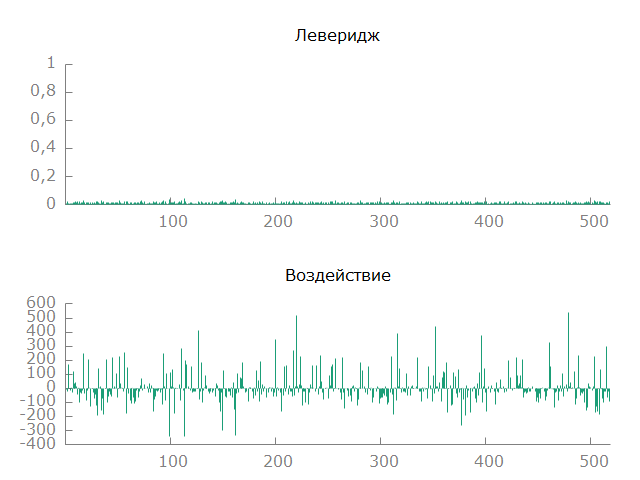
\includegraphics[width=0.7\textwidth]{../[graphics]/lever.png}
	\centering
	\caption{Графики Леверижда и Воздействия}
	\label{fig:lever}
\end{figure}

В соответствии с литературой\footnote{%
Fox J. Quantitative applications in the social sciences, No. 79. Regression diagnostics. – 1991.}, выброс регресии - это наблюдение, для которого значение стоимости страховки исключительно высоко или низко при заданных независимых переменных. Редким значением называется исключительно низкое или высокое значение зависимой или независимой переменной некоторого объекта. 

В соответствии c графиком Леверижда (рис. \ref{fig:lever}) видно, что все объекты в равной степени влияют на уравнение регрессии. Выделим в отдельную таблицу объекты (выбросы), соответствующие точкам разбалансировки, которые выделяются на фоне других значений Леверижда.
О потенциальных выбросах можно говорить и при анализе статистики Воздействия. Объекты с большим значением статистики Воздействия также занесем в таблицу и дополнительно проанализируем.

\begin{table}[H]
	\begin{center}
	\begin{tabular}{|l|l|l|l|l|l|l|}
		\hline
		№ наблюдения & age & sex      & bmi    & children & smoker & charges  \\ \hline
		35.  & 59  & "male"   & 29,830 & 3        & "yes"  & 30184,94 \\ \hline
		52.  & 32  & "female" & 17,765 & 2        & "yes"  & 32734,19 \\ \hline
		94.  & 23  & "female" & 36,670 & 2        & "yes"  & 38511,63 \\ \hline
		99.  & 18  & "male"   & 17,290 & 2        & "yes"  & 12829,46 \\ \hline
		111.  & 54  & "male"   & 40,565 & 3        & "yes"  & 48549,18 \\ \hline
		114.  & 46  & "female" & 48,070 & 2        & "no"   & 9432,93  \\ \hline
		150.  & 27  & "female" & 17,955 & 2        & "yes"  & 15006,58 \\ \hline
		162.  & 26  & "female" & 17,195 & 2        & "yes"  & 14455,64 \\ \hline
		217.  & 48  & "male"   & 40,565 & 2        & "yes"  & 45702,02 \\ \hline
		377. & 27  & "female" & 20,045 & 3        & "yes"  & 16420,49 \\ \hline
		503. & 62  & "male"   & 30,875 & 3        & "yes"  & 46718,16 \\ \hline
	\end{tabular}
\caption{Выбросы}
\label{tab:out}
	\end{center}
\end{table}

Удалим указанные в таблице \ref{tab:out} наблюдения из выборки и построим модель для проверки 2 гипотезы заново.

\begin{table}[H]
\begin{center}
	bmi\_model\_without\_outliers:
	МНК, использованы наблюдения 1--507\\
	Зависимая переменная: charges\\
	\vspace{1em}
	\begin{tabular}{|l|r@{,}l|r@{,}l|r@{,}l|r@{,}l|}
		\hline
		&
		\multicolumn{2}{c|}{Коэффициент} &
		\multicolumn{2}{c|}{Ст.\ ошибка} &
		\multicolumn{2}{c|}{$t$-статистика} &
		\multicolumn{2}{c|}{P-значение} \\[1ex] \hline
		const &	$-$6775&18 & 2412&94 & $-$2&808 & 0&0052 \\ \hline
		age & 247&622 & 18&5428 & 13&35 & 0&0000 \\ \hline
		bmi & 131&319 & 91&2360 & 1&439 & 0&1507 \\ \hline
		Dchildren\_2 & 1451&55 & 707&881 & 2&051 & 0&0408 \\ \hline
		Dchildren\_many & 2001&69 & 725&302 & 2&760 & 0&0060 \\ \hline
		Dsmoker\_2 & 21349&5 & 677&309 & 31&52 & 0&0000 \\ \hline
		bmi\_bmi\_ind & 85&0571 & 28&4498 & 2&990 &	0&0029 \\ \hline
	\end{tabular}
	\vspace{1ex}
	\begin{tabular}{lrlr}
		Среднее зав. перемен &  12523,96 & Ст. откл. зав. перемен &  10770,07 \\
		Сумма кв. остатков &  1,69\textrm{e+10} & Ст. ошибка модели &  5808,228 \\
		$R^2$ &  0,712611 & Исправленный $R^2$ &  0,709163 \\
		$F(6, 500)$ &  206,6340 & Р-значение($F$) &  6,7\textrm{e--132} \\
		Лог. правдоподобие & $-$5110,062 & Крит. Акаике &  10234,12 \\
		Крит. Шварца &  10263,72 & Hannan--Quinn &  10245,73 \\
	\end{tabular}
\caption{Модифицированная модель для проверки гипотезы 2 с удаленными выбросами}
\label{model-out}
\end{center}
\end{table}

Из таблицы \ref{model-out} видно, что значение константы существенно увеличилось (выбросы больше не смещают модель в сторону больших значений страховых взносов), надбавка за двух детей значительно увеличилась (при фиксированных значениях остальных показателей), а переменная bmi стала незначимой.

\subsection{Анализ наличия гетероскедастичности}
\begin{table}[H]
	\begin{center}
		\begin{tabular}{ | l | l |}
			\hline
			Тестовая статистика: & $TR^2 = 72,926667$ \\ \hline
			р-значение: & $P$(Хи-квадрат($22$) $> 72,926667$) = $0,000000$ \\ \hline
		\end{tabular}
	\end{center}
	\caption{Тест Вайта (White) на гетероскедастичность}
	\label{tab:white}
\end{table}

В соответствии с таблицей \ref{tab:white} нами отвергается нулевая гипотеза об отсутствии гетероскедастичности в модифицированной модели для проверки 2 гипотезы - она является лучшей моделью согласно следующему пункту. Гетероскедастичность есть (не выполняется предположение о том, что дисперсии случайных составляющих совпадают). Стандартные ошибки могут быть подсчитаны неправильно. Воспользуемся корректировкой Вайта для решения этой проблемы:

\begin{table}[H]
\begin{center}
	bmi\_model\_2:
	МНК, использованы наблюдения 1--518\\
	Зависимая переменная: charges\\
	Робастные оценки стандартных ошибок (с поправкой на гетероскедастичность),\\ вариант HC0\\
	\vspace{1em}
	\begin{tabular}{|l|r@{,}l|r@{,}l|r@{,}l|r@{,}l|}
		\hline
		&
		\multicolumn{2}{c|}{Коэффициент} &
		\multicolumn{2}{c|}{Ст.\ ошибка} &
		\multicolumn{2}{c|}{$t$-статистика} &
		\multicolumn{2}{c|}{P-значение} \\[1ex] \hline
		const &	$-$8226&27 & 2238&05 & $-$3&676 & 0&0003 \\ \hline
		age & 252&679 &	18&1944 & 13&89 & 0&0000 \\ \hline
		bmi & 176&827 &	87&4791 & 2&021 & 0&0438 \\ \hline
		Dchildren\_2 & 1328&85 & 770&668 & 1&724 & 0&0853 \\ \hline
		Dchildren\_many & 2020&65 &	723&991 & 2&791 & 0&0055 \\ \hline
		Dsmoker\_2 & 21362&3 & 905&057 & 23&60 & 0&0000 \\ \hline
		bmi\_bmi\_ind & 79&9783 & 27&9858 &	2&858 &	0&0044 \\ \hline
	\end{tabular}
	\vspace{1ex}
	\begin{tabular}{lrlr}
		Среднее зав. перемен &  12857,52 & Ст. откл. зав. перемен &  11094,27 \\
		Сумма кв. остатков &  1,77\textrm{e+10} & Ст. ошибка модели &  5881,548 \\
		$R^2$ &  0,722210 & Исправленный $R^2$ &  0,718949 \\
		$F(6, 511)$ &  141,0821 & Р-значение($F$) &  5,0\textrm{e--105} \\
		Лог. правдоподобие & $-$5227,506 & Крит. Акаике &  10469,01 \\
		Крит. Шварца &  10498,76 & Hannan--Quinn &  10480,67 \\
	\end{tabular}
\caption{Модифицированная модель для проверки гипотезы 2 с поправкой на гетероскедастичность}
\end{center}
\end{table}


\subsection{Оптимизация модели}
\begin{table}[H]
	\begin{center}
		\begin{tabular}{ | l | l | l | l |}
			\hline
			Модель/Критерий & $R^2$ & $Adj R^2$ & $Akaike$ \\ \hline
			1. Базовая модель & $0,717829$ & $0,715074$ & $10475,12$ \\ \hline
			2. Модифицированная модель 1 & $0,722210$ & $0,718949$ & $10469,01$ \\ \hline
			3. Модифицированная модель 2 & $0,722277$ & $0,718465$ & $10470,89$ \\ \hline
			4. Модифицированная модель 1 без выбросов & $0,712611$ & $0,709163$ & $10234,12$ \\ \hline
		\end{tabular}
	\end{center}
	\caption{Результаты анализа оптимальности построенных моделей}
	\label{tab:optim}
\end{table}

Анализируя таблицу \ref{tab:optim}, можно заметить, что в соответствии с показателем $Adj. R^2$ (наибольшее значение) модифицированная модель для проверки гипотезы 2 является лучшей. Это объясняется тем, что у базовой модели не было учтено увеличение скорости роста цены после некоторого значения ИМТ - данная зависимость дает прирост в качестве. В то же время модель 3 содержала дополнительную незначимую переменную (критерий $R^2$ наибольший у модели 3), что отразилось на значениях $Adj. R^2$ и Акаике. В модифицированной модели 1 без выбросов значение критерия Акаике наилучшее (наименьшее значение), но остальные показатели наихудшие.

\section{Выводы и рекомендации}
Определим минимальный индивидуальный взнос для некурящих женщин в возрасте 19-44 лет с ИМТ в диапазоне от 18,5 до 25 при наличии двух детей. Как было выявлено, размер страхового взноса не зависит от пола. Минимальный взнос будет достигнут в возрасте 19 лет со значением ИМТ 18,5 и равен $-8226,27 + 252,679 * 19 + 79,9783 * 0 + 176,827 * 18,5 + 1328,85 * 1  + 2020,65 * 0 + 21362,3 * 0 = 1174,7805$ долларов.

С использованием построенной модели потребитель сможет оценивать размер страховых взносов человека, основываясь на его индивидуальных характеристиках. 

В результате проверки было выявлено, что наличие вредных привычек сильно увеличивает стоимость страховки. Кроме того, выделен линейный рост стоимости страховки с увеличением возраста, причем для мужчин скорость роста такая же, как и для женщин. Зависимость цены взносов от ИМТ более сложная, после значения ИМТ, равного 30, сила его влияния на цену увеличивается.

\begin{figure}[H]
	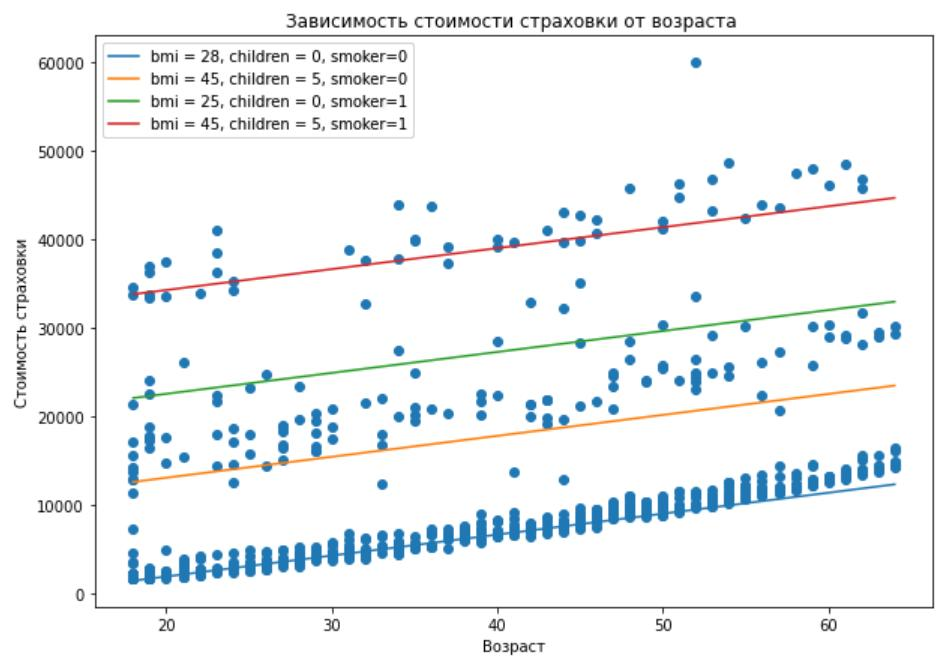
\includegraphics[width=0.7\textwidth]{../[graphics]/example.jpg}
	\centering
	\caption{Зависимость цены страховки от возраста}
	\label{fig:example}
\end{figure}

Также были проиллюстрированы изменения в стоимости страховки с возрастом при некоторых фиксированных показателях (рис. \ref{fig:example}). Нижняя линия описывает человека с нормальным значеним ИМТ, некурящего и без детей. Зеленая линия описывает человека с нормальным значеним ИМТ без детей, но курящего. Видно, что цена страховки колоссально отличается. Оранжевая линия соответствует некурящему человеку, но с сильным ожирением и большим количеством детей. Тем не менее, стоимость его страховки меньше, чем у курящего человека с нормальным ИМТ и без детей. Красная линия, описывающая максимальную стоимость за страховку, соответствует человеку курящему, с сильным ожирением и большим числом детей.
\end{document} % конец документа